\documentclass[tikz,border=5mm]{standalone}

\usepackage{tikz}
\usetikzlibrary{trees}
\usetikzlibrary{positioning}

\begin{document}

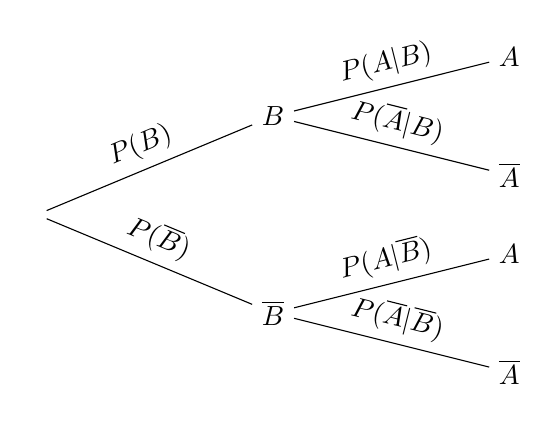
\begin{tikzpicture}[
        level distance=3cm,
        level 1/.style = {sibling distance=2.5cm},
        level 2/.style = {sibling distance=1.5cm},
        grow'=right,
        sloped
    ]
    \node (Root) {}
    child {
            node  {$B$}
            child {
                    node {$A$}
                    edge from parent
                    node[above] {$P(A|B)$}
                }
            child {
                    node {$\overline{A} $}
                    edge from parent
                    node[above] {$P(\overline{A} | B)$}
                }
            edge from parent
            node[above] {$P(B)$}
        }
    child {
            node {$\overline{B}$}
            child {
                    node {$A$}
                    edge from parent
                    node[above] {$P(A|\overline{B})$}
                }
            child {
                    node {$\overline{A} $}
                    edge from parent
                    node[above] {$P(\overline{A}|\overline{B})$}
                }
            edge from parent
            node[above] {$P(\overline{B})$}
        }
    ;
\end{tikzpicture}

\end{document}
